\documentclass[dwyatte_dissertation.tex]{subfiles} 
\begin{document}

\chapter{Spatial and temporal prediction during novel object recognition: \\ Temporal and spectral signatures}
\label{chap:pleast}

\section{Introduction}
TODO, pull from proposal and proposal-r1. Try to write without referencing LeabraTI too much, this chapter should stand by itself

\section{Methods}

\subsection{Participants}
% 29 D464B EEG 
% 29 Behavioral only
% ===
% 58 total, 27 female (ages 18-28 mean=21)
A total of 58 students from the University of Colorado Boulder participated in the experiment (ages 18-28 years, mean=21; 31 male, 27 female). EEG was recorded from 29 of the participants while they completed the experiment. The remaining 29 participants completed a solely behavioral experiment without EEG recording. All participants were right-handed and reported normal or corrected-to-normal vision. Participants either received course credit or payment of \$15 per hour as compensation for their participation. Informed consent was obtained from each participant prior to the experiment in accordance with Institutional Review Board policy at the University of Colorado.

\subsection{Stimuli}
Novel ``paper clip'' objects similar to those used in previous studies \cite{BulthoffEdelman92,EdelmanBulthoff92,LogothetisPaulsBulthoffEtAl94,LogothetisPaulsPoggio95,SinhaPoggio96} were created using MATLAB. Eight vertices were placed randomly on the surface of a sphere of unit radius and then joined together with line segments. The last and first vertex were also joined to form a closed loop so that line segment terminations were not a salient feature \cite{BalasSinha09b}. Objects were constrained to exclude extremely acute angles between successive segments (less than 20 degrees) and were approximately rotationally balanced (center of mass within 10\% of the origin). Objects were were rotated completely about their vertical axis in steps of 12 degrees and rendered to bitmap images under an orthographic projection. A total of 16 objects were created using this procedure, yielding 480 images (30 images per object). Object examples are shown in Figure \ref{fig:pleast_objs}.

% paperclip fig
% rotations for one obj, several objs
\begin{figure}[h!]
\begin{center}
\begin{tabular}{ll}
\textbf{A} \\
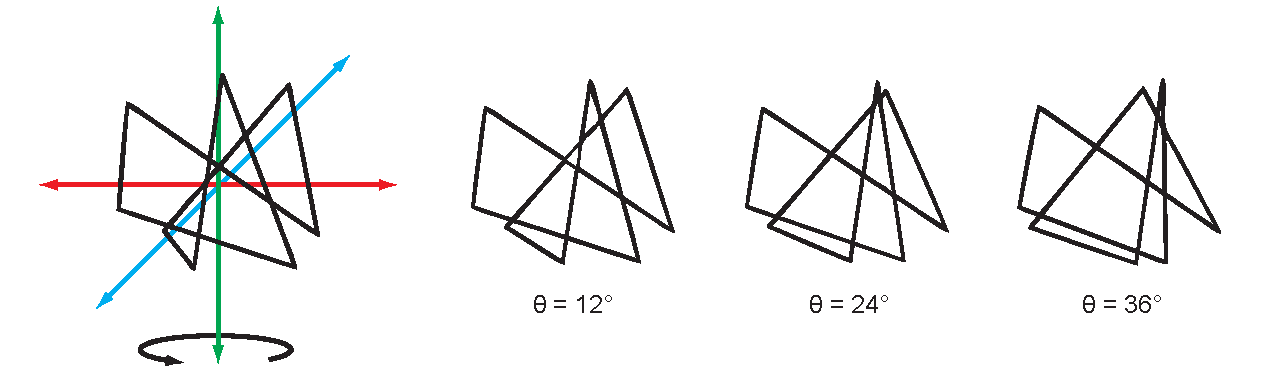
\includegraphics[width=160mm]{figs/chap_pleast/paperclip_rots.pdf} \\
\textbf{B} \\
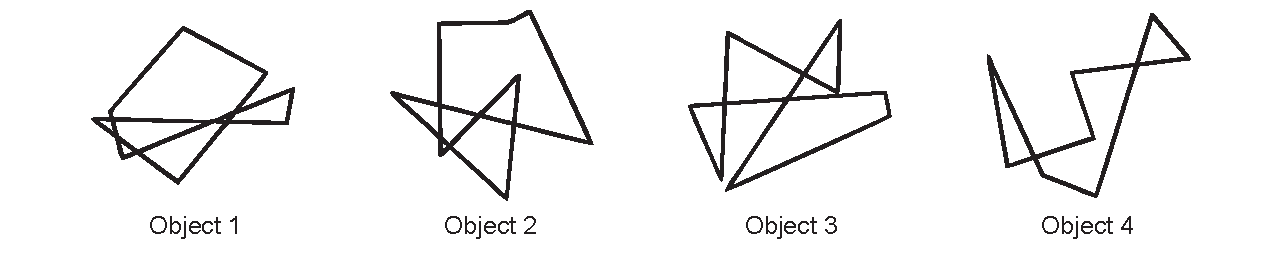
\includegraphics[width=160mm]{figs/chap_pleast/paperclip_objs.pdf} \\
\end{tabular}
\end{center}
\caption{Novel ``paper clip'' objects}{\textbf{A:} Objects were composed of eight three-dimensional vertices joined together with line segments. To render the objects to bitmap images, each object was rotated completely about its vertical axis in steps of 12 degrees and reduced to an orthographic projection. \textbf{B:} Four of the 16 objects used in the experiment.}
\label{fig:pleast_objs}
\end{figure}

\subsection{Procedure}
Participants observed an entraining sequence of rotated views of a random object and performed a same-different judgement about a probe stimulus. On each trial, a view was randomly selected as the initial view of the sequence followed by seven additional views spaced 24 degrees apart (Figure \ref{fig:pleast_task}A, blue tick marks). Thus, the eight view entraining sequence spanned 168 degrees of the object. The entraining sequence was either presented in order (i.e., spatially predictable) or randomized. Following the entraining sequence after a 200 ms blank was a probe stimulus consisting of either an unseen view from the entraining object or a novel distractor. Unseen views were randomly sampled from the 12 degree interpolations between views of the entraining sequence (Figure \ref{fig:pleast_task}A, magenta tick marks) and from outside of the span of the entraining sequence in increments of 24 degrees (Figure \ref{fig:pleast_task}A, green tick marks).

Distractors were created from the original target objects by randomly selecting new spherical coordinates for six of the eight vertices and re-rendering them to bitmap images using the same method as the original target objects (12 degree steps about the vertical axis). Distractors conformed to the same constraints as the original target objects (no extremely acute angles, approximately rotationally balanced). Participants were instructed to respond ``same'' if they believed the probe depicted the same object as the entraining sequence or ``different'' if it depicted a distractor object. Participants received feedback after each trial according to whether their response was correct or incorrect. % Responses were collected via a millisecond-accurate response box connected through the display computer's serial port. 

During the entraining sequence, object views were presented for 50 ms at either 10 Hz (i.e., temporally predictable) or at a variable rate by manipulating the interstimulus interval (ISI) between subsequent views. Temporally predictable ISIs were 50 ms, totaling 350 ms across the entraining sequence. Variable ISIs were selected by randomly generating seven ISIs that also summed to 350 ms (Figure \ref{fig:pleast_task}B). ISIs were in the range of 16.67 ms (minimum) to 216.67 ms (maximum) in increments of 16.67 ms. Temporal unpredictability was maximized by generating 400 such ISI sequences, calculating the summed squared error (SSE) across subsequent ISIs in a sequence, and selecting the 100 sequences with the highest SSE for use during the experiment.

% task fig
\begin{figure}[h!]
\begin{center}
\begin{tabular}{ll}
\textbf{A} \\
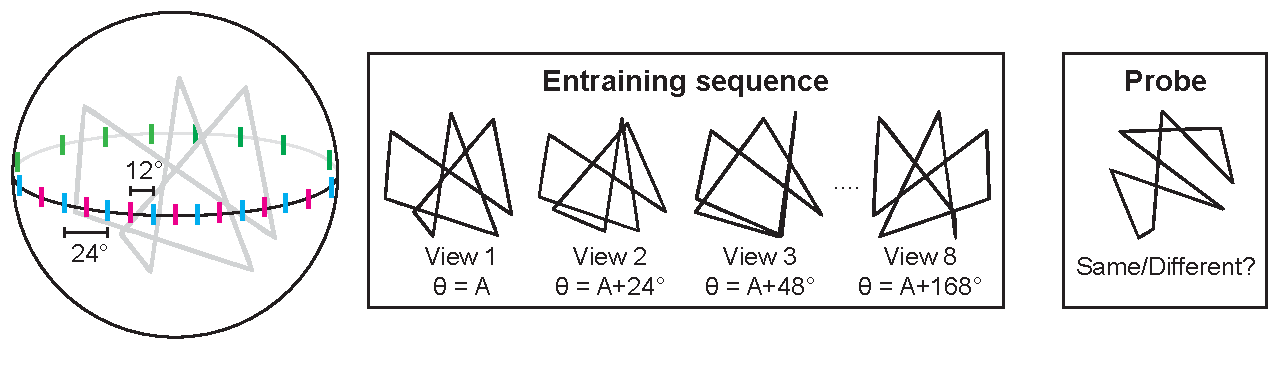
\includegraphics[width=160mm]{figs/chap_pleast/paperclip_task.pdf} \\
\textbf{B} \hspace{90mm} \textbf{C} \\
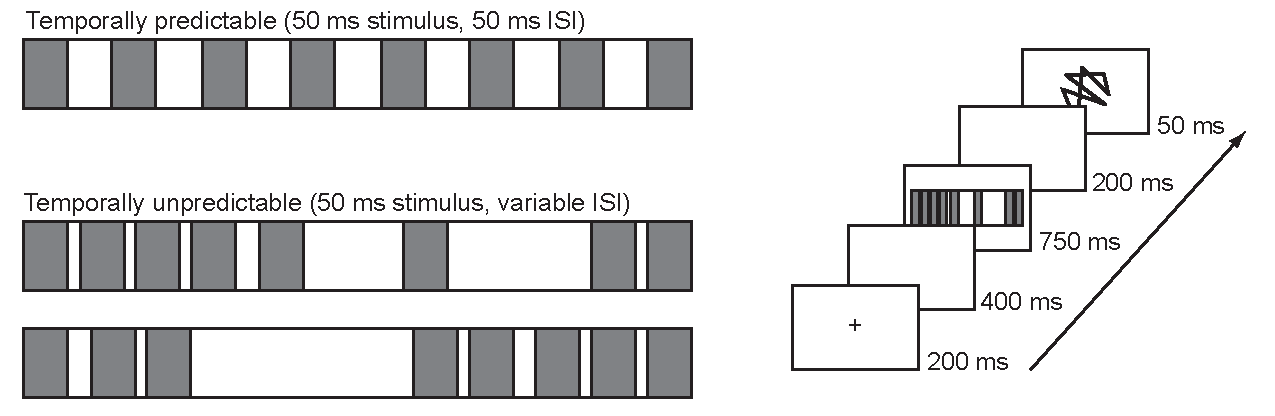
\includegraphics[width=160mm]{figs/chap_pleast/paperclip_ISI.pdf} \\
\end{tabular}
\end{center}
\caption{Experimental procedure}{\textbf{A:} Experimental trials contained an entraining sequence composed of eight views of a single object, followed by a probe stimulus. Entraining views were spaced 24 degrees apart (blue tick marks). The probe depicted an unseen view from the 12 degree interpolations between views of the entraining sequence (magenta tick marks) or from outside the span of the entraining sequence in increments of 24 degrees (green tick marks). \textbf{B:} Entraining views were either presented at 10 Hz with a 50 ms on time and 50 ms off time or in a temporally unpredictable manner with a 50 ms on time (gray segments) and variable off time (white segments). In both cases, the duration of the total entraining sequence was held constant at 750 ms. \textbf{C:} Order and timing  of events within a single trial.}
\label{fig:pleast_task}
\end{figure}

The experiment was displayed on an LCD monitor at native resolution operating at 60 Hz using the Psychophysics Toolbox Version 3 \cite{Brainard97,Pelli97}. Stimuli were presented on an isoluminant 50\% gray background and subtended approximately 5 degrees of visual angle. Trials began with a fixation cross (200 ms) followed by a blank (400 ms), the entraining sequence (750 ms total), a second blank (200 ms), and ended with the probe stimulus (50 ms) (Figure \ref{fig:pleast_task}C). Participants were required to respond within 2000 ms. Trials were separated by a variable intertrial interval of 2000-2400 ms. The experiment contained 500 trials with an additional 20 practice trials that contained a longer blank (1000 ms) between the entraining sequence and the probe to familiarize participants with the order of events during trials. Participants completed the 20 practice trials (which were discarded from analysis) prior to performing the 500 experimental trials. % random sampling of all variables with replacement

\subsection{EEG recording and preprocessing}
% Net Station 4.3.1
The EEG was recorded using an Electrical Geodesics, Inc. (EGI) system composed of a 128 channel net (HCGSN 130) amplified through 200 M\SI{}{\ohm} amplifiers (Net Amps 200). The signal was sampled at 250 Hz with impedances for each electrode were adjusted to less than 40 k\SI{}{\ohm} before and during the recording. Stimulus and response trigger onsets were measured via the Psychophysics Toolbox using a high precision realtime clock that was synchronized within 2.5 ms of the EEG system's clock before every trial during the experiment.

EEG data were preprocessed using the FieldTrip toolbox \cite{OostenveldFriesMarisEtAl11}. Raw data were first band-pass filtered between 1 Hz and 100 Hz with a 59-61 Hz band-stop and then epoched into 2350 ms segments that spanned the start of the pre-trial blank to 1000 ms after the probe stimulus. Individual segments were visually inspected and rejected if found to contain muscle artifacts or atypical noise. Bad channels were also identified and temporarily removed from the data before performing ICA decomposition \cite{DelormeMakeig04} to remove of ocular artifacts. Components related to ocular artifacts were identified based on their topographical distribution across electrodes. The data were reconstructed without the ocular components and any bad channels were replaced using spherical spline interpolation \cite{PerrinPernierBertrandEtAl89}. The resulting segments were re-referenced to the average reference.

\subsection{Event-related averaging}
Event-related averaging was performed separately for the entraining sequence and the subsequent probe. For the entraining sequence, data were aligned to the onset of entraining views 2 through 8 and averaged from the period beginning 50 ms before each entrainer and ending 50 ms after. Baseline correction was performed using the first 50 ms of this period. For the probe, data were aligned to the probe onset and averaged from the period beginning 200 ms before the probe and ending 400 ms after. This allowed detection of predictability effects during the blank period due to differences in phase elicited by the entraining sequence as well as probe-evoked predictability effects.

All waveforms were averaged over a montage of 23 electrodes that covered the occipital and parietal cortices (Figure \ref{fig:pleast_channels}). The montage included locations from the 10-10 system that are commonly associated with perceptual processing (Oz, O1/O2, PO3/PO4, and PO7/PO8) \cite[e.g.,]{DohertyRaoMesulamEtAl05,RohenkohlNobre11,FahrenfortScholteLamme07}.

% electrode poolings fig
\begin{figure}[h!]
\begin{center}
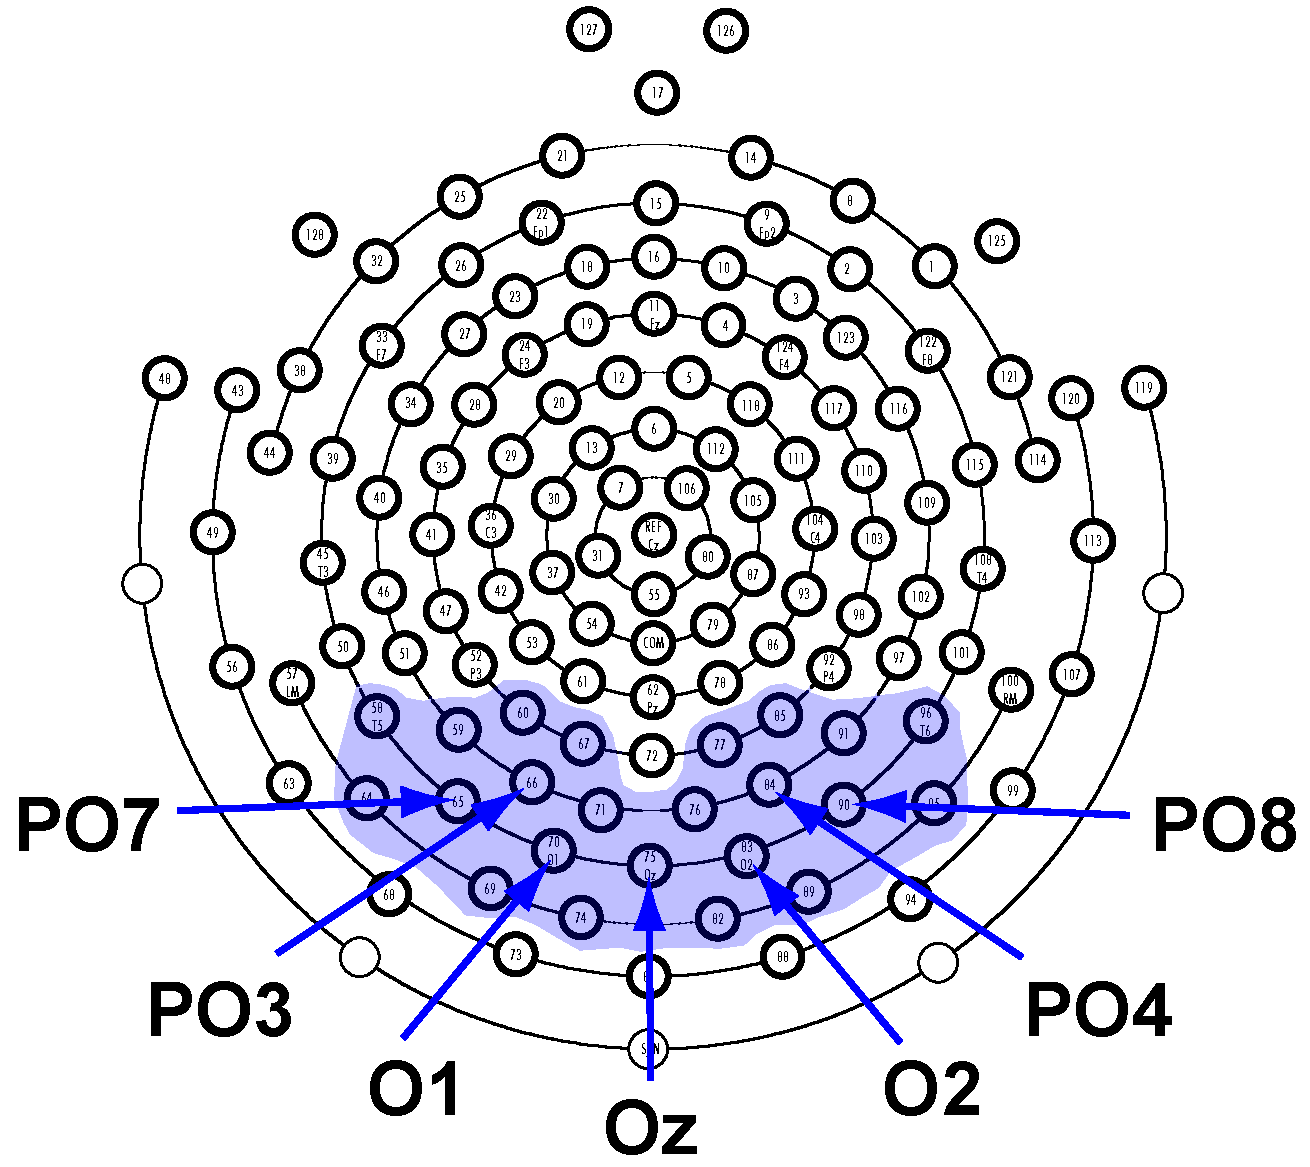
\includegraphics[width=80mm]{figs/chap_pleast/channels_all.pdf}
\end{center}
\caption{Electrode pooling for analyses}{Blue shaded region denotes pooled electrodes. Locations from the 10-10 system are indicated.}
\label{fig:pleast_channels}
\end{figure}

\subsection{Time-frequency analysis}
Segmented data were used to compute time-frequency data for each trial. Data were first downsampled to 125 Hz and then used to compute the instantaneous Fourier coefficients at each time bin using a multi-taper approach. Hanning tapers were generated at 5-40 Hz and convolved with the data using a sliding time window (four cycles per frequency per time window). The relatively long time window required for low-frequency bands prevents computation of time-frequency data for short time segments, such as the 200 ms blank before the probe. To address this issue, time-frequency data was computed over the entire 2350 ms trial epoch and then cropped to investigate temporal regions of interest.

Power was computed from the magnitude of the instantaneous Fourier coefficients at each frequency (\textit{f}) and time bin (\textit{t}):w
\begin{align*}
Power(f,t) = \frac{1}{n} \sum_{k=1}^{n}{|F_k(f,t)|}^2
\end{align*}

Phase, which is normally defined as the angle of the complex Fourier coefficients, cannot be averaged due to its circularity and thus standard statistical models cannot be applied to assess its significance. One solution to this problem is to compute inter-trial coherence (ITC) instead \cite{LachauxRodriguezMartinerieEtAl99}. ITC is averaged in the complex domain by first normalizing phase information to unit length by dividing off power and computing the magnitude:
\begin{align*}
ITC(f,t) = \bigg{|}\frac{1}{n} \sum_{k=1}^{n}{\frac{F_k(f,t)}{|F_k(f,t)|}}\bigg{|}
\end{align*}

ITC ranges between 0 and 1 and represents how systematic phase angles are across trials. A value of 0 indicates that phase information is essentially uniformly distributed across trials while a value of 1 indicates a high degree of phase-locking at a particular frequency across trials.

All time-frequency analyses were averaged over the same montage of 23 occipitoparietal electrodes that was used to compute event-related averages (Figure \ref{fig:pleast_channels}). 

\section{Results}

\subsection{Behavioral measures of spatial and temporal predictability}
% timeouts removed from data
Five subjects were excluded from behavioral analysis for accuracy 2.7$\sigma$ (or further) below mean accuracy across subjects. The remaining 53 subjects were submitted to a 2x2 ANOVA with spatial and temporal predictability as within-subjects factors. Experiment type (EEG or behavioral only) was included as an additional between-subjects factor to ensure that it did not interact with any of the within-subjects factors. Accuracy and reaction times were collected during the experiment and were used to compute \textit{d'}, a measure of sensitivity that takes into account response bias, and inverse efficiency, a measure that combines accuracy and reaction times \cite{TownshendAshby78}. These behavioral measures are plotted in Figure \ref{fig:pleast_behave}.

% oh, behave
\begin{figure}[h!]
\begin{center}
\begin{tabular}{ll}
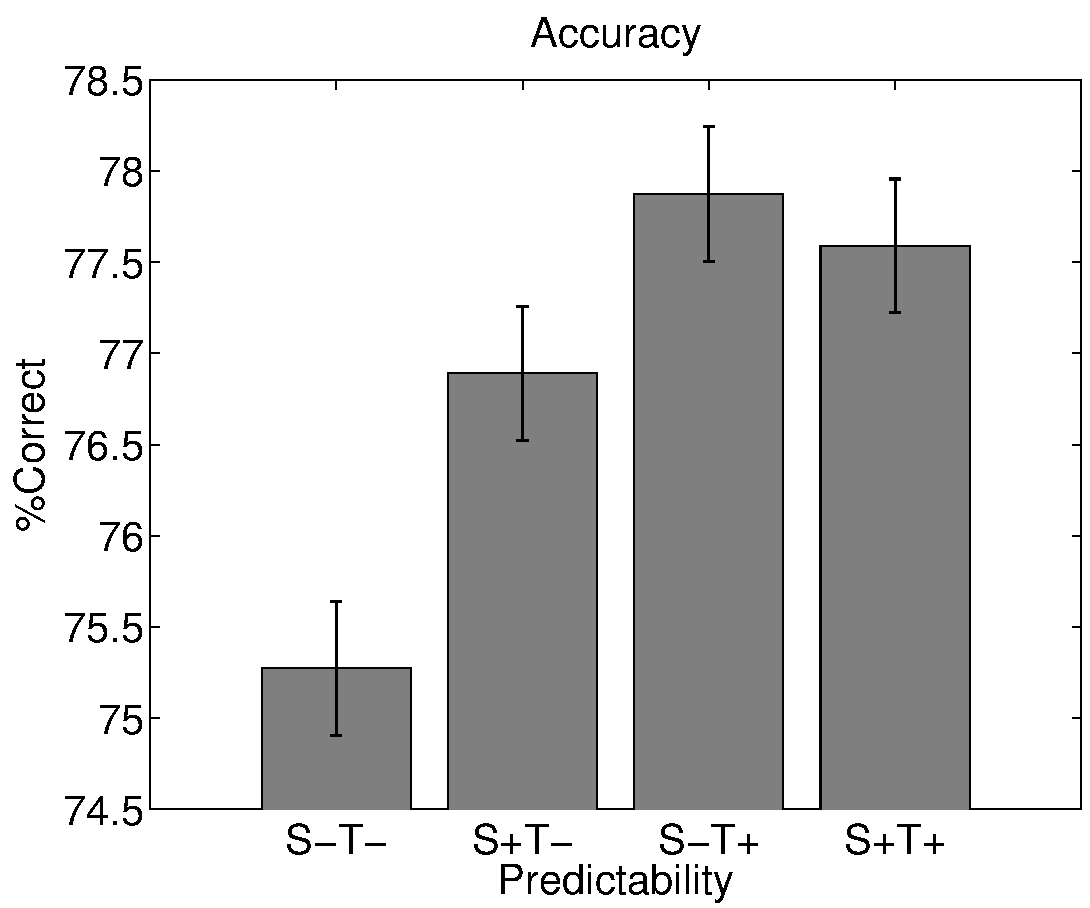
\includegraphics[width=80mm]{figs/chap_pleast/results_accuracy.pdf} & 
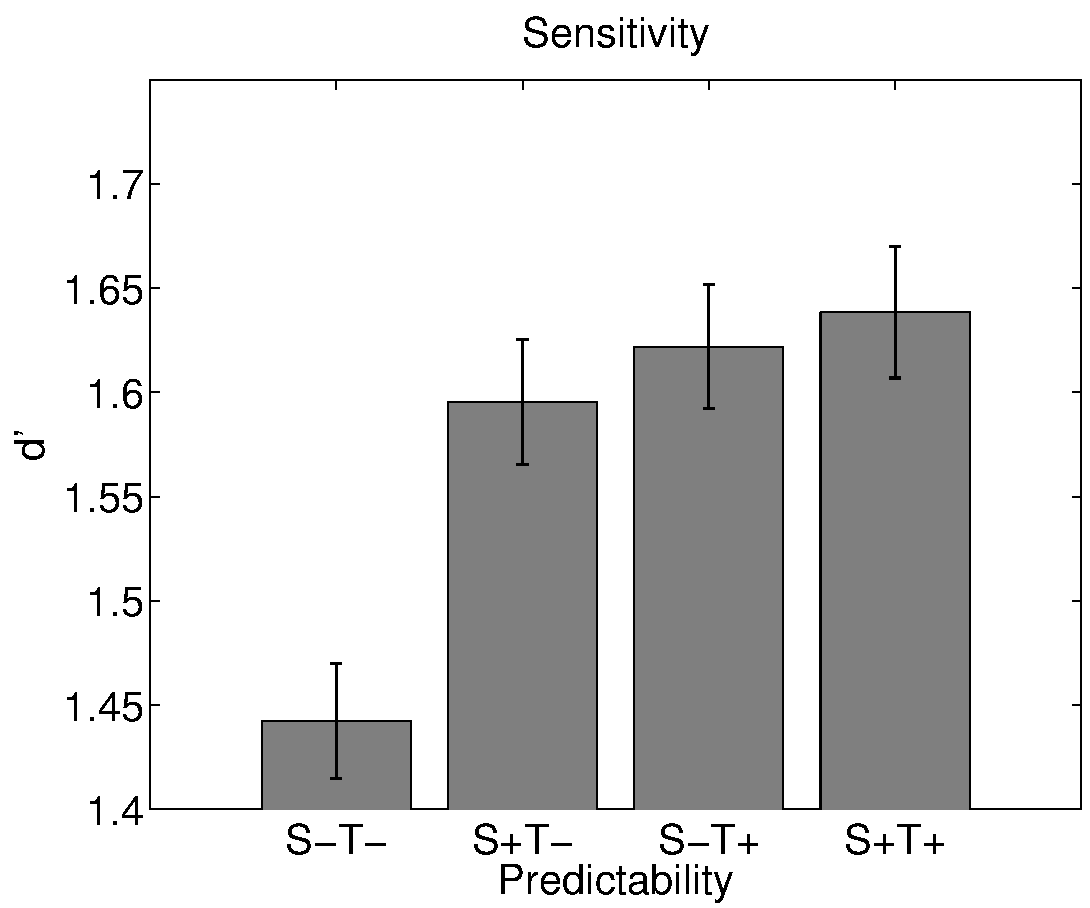
\includegraphics[width=80mm]{figs/chap_pleast/results_dprime.pdf} \\
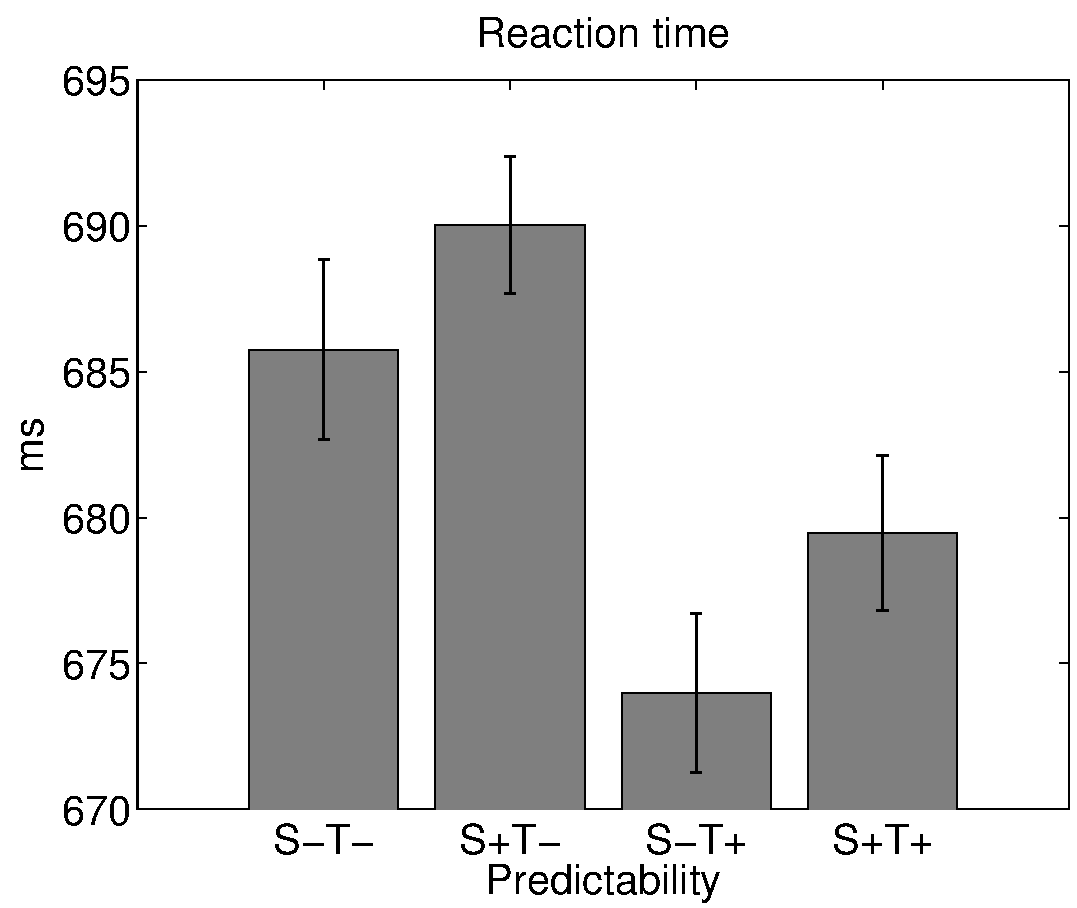
\includegraphics[width=80mm]{figs/chap_pleast/results_rt.pdf} &
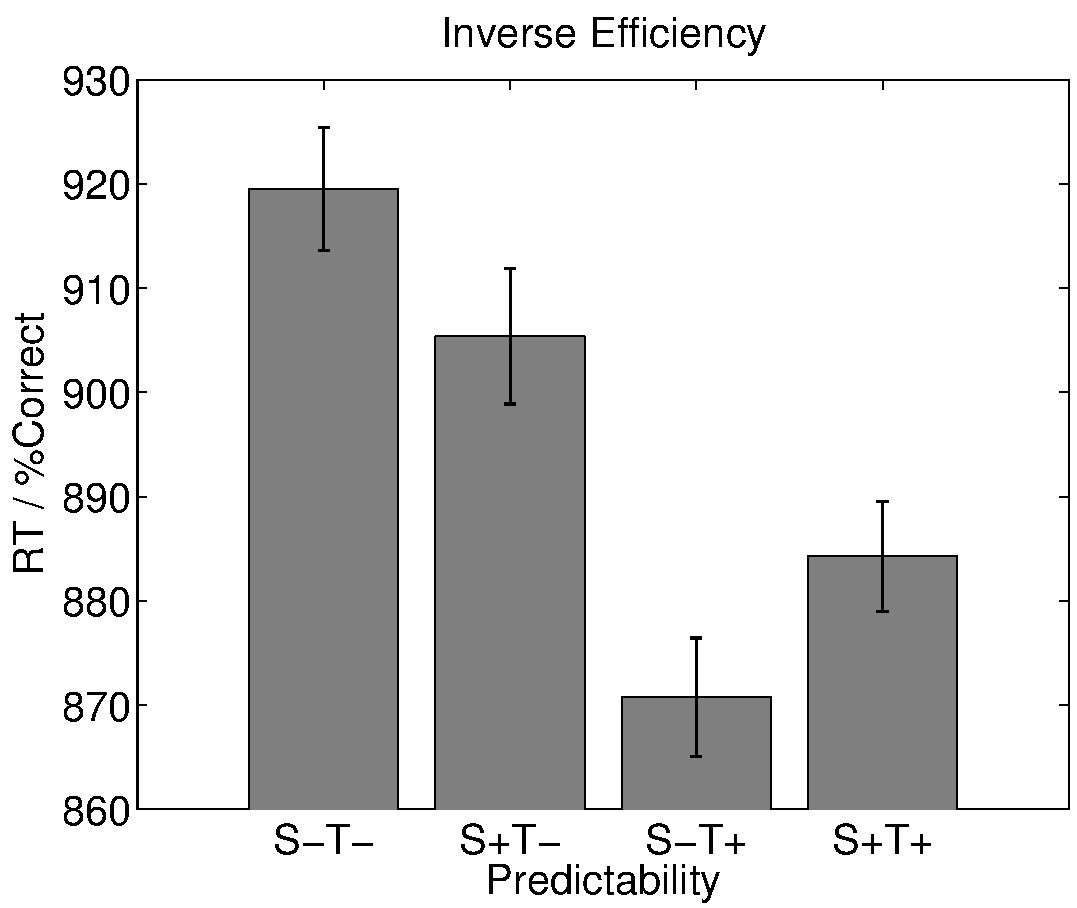
\includegraphics[width=80mm]{figs/chap_pleast/results_ie.pdf} \\
\end{tabular}
\end{center}
\caption{Behavioral measures of spatial and temporal predictability}{Accuracy, \textit{d'} (sensitivity), reaction time, and inverse efficiency (reaction time divided by percent correct) as a function of entrainment condition. S-/+ refers to spatially unpredictable and predictable, T-/+ to temporally unpredictable and predictable. Error bars depict within-subjects error using the method described in \protect\incite{Cousineau05} adapted for standard error.}
\label{fig:pleast_behave}
\end{figure}

% D464B subs acc=75, rt=624.72
% E029 subs acc=0.79 rt=742.1212
Subjects that completed the full EEG experiment were on average less accurate (\textit{F}(1, 51) = 4.80, \textit{p} = 0.033) but responded more quickly (\textit{F}(1, 51) = 10.05, \textit{p} = 0.003) than subjects that completed the solely behavioral experiment. These differences reflect a speed-accuracy tradeoff, likely due to differences in instructions given to subjects by experimenters or motivational differences between subject groups. Importantly, experiment type did not interact with any within-subjects factors (all \textit{p}'s $>$ 0.05) indicating that the behavioral measures of interest were not dependent on which type of experiment subjects completed.

Overall, subjects were more accurate when the entraining sequence was temporally predictable (\textit{F}(1, 51) = 17.84, \textit{p} $<$ 0.001). A similar effect for spatial predictability failed to reach significance (\textit{F}(1, 51) = 1.85, \textit{p} = 0.18). The interaction between spatial and temporal predictability, however, was significant (\textit{F}(1, 51) = 6.13, \textit{p} = 0.017). The LeabraTI model (Chapter \ref{chap:leabrati}) as well as previous investigations of predictability \cite[e.g.,]{DohertyRaoMesulamEtAl05} suggest that spatial and temporal predictability should have an additive effect on behavioral outcomes. However, the combined spatial and temporal predictability condition here (denoted S+T+ in Figure \ref{fig:pleast_behave}) is sub additive. Although not significantly different from spatial predictability alone (\textit{t}(52) = 1.29, \textit{p} = 0.204) or from temporal predictability alone (\textit{t}(52) = 0.45, \textit{p} = 0.652), this result merits further investigation. 

When responses are transformed into \textit{d'}, there is a significant effect of both spatial (\textit{F}(1, 51) = 4.71, \textit{p} = 0.035) and temporal predictability (\textit{F}(1, 51) = 11.99, \textit{p} $<$ 0.001). This result suggests that response bias can at least partially explain why spatial predictability failed to reach significance for raw accuracy. The interaction between spatial and temporal predictability remained significant for \textit{d'} (\textit{F}(1, 51) = 4.49, \textit{p} = 0.039). The interaction is additive, but is driven primarily by the strong effect of introducing spatial or temporal predictability over complete unpredictability (S-T- versus S+T-, \textit{t}(52) = 3.19, \textit{p} = 0.002; S-T- versus S+T+, \textit{t}(52) = 4.26, \textit{p} $<$ 0.001) opposed to any synergistic effect of combined spatial and temporal predictability (S+T+ versus S+T-, \textit{t}(52) = 0.90; S+T+ versus S-T+, \textit{t}(52) = 0.31; both \textit{p}'s $>$ 0.05).

Reaction times were significantly faster when the entraining sequence was temporally predictable (\textit{F}(1, 51) = 12.38, \textit{p} $<$ 0.001). A similar effect for spatial predictability failed to reach significance (\textit{F}(1, 51) = 1.96, \textit{p} = 0.168) nor did the interaction term (\textit{F}(1, 51) = 0.05, \textit{p} = 0.83).

Inverse efficiency, which considers reaction time as a function of accuracy (defined as reaction time divided by percent correct) can be thought of as the amount of energy consumed by the system to produce a behavioral outcome \cite{TownshendAshby83}. It is often used to remove non-monotonicities present in accuracy or reaction times alone, although that effect is not observed here. Nevertheless, it provides another lens under which to interpret the results, and thus it is considered here. Inverse efficiency was significantly lower when the entraining sequence was temporally predictable (\textit{F}(1, 51) = 23.31, \textit{p} $<$ 0.001), but not when it was spatially predictability (\textit{F}(1, 51) = 0.002, \textit{p} = 0.963). Inverse efficiency is characterized by a significant cross-over interaction (\textit{F}(1, 51) = 5.85, \textit{p} = 0.019). Spatial predictability of the entraining sequence produces lowers inverse efficiency over complete unpredictability. Inverse efficiency is lowest on average when stimuli are temporally predictable, but the addition of spatial predictability causes an increase in inverse efficiency.

%% oh, behave pt 2
%\begin{figure}[h!]
%\centering
%\begin{tabular}{ll}
%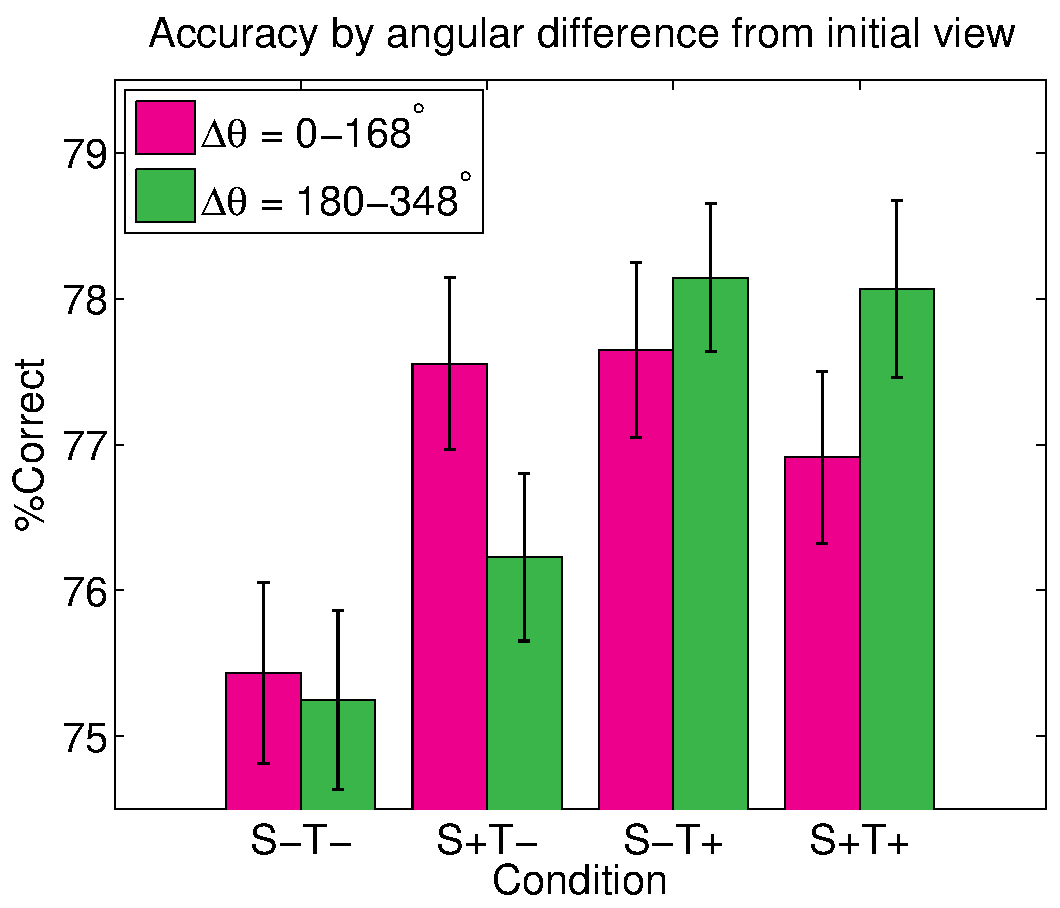
\includegraphics[width=80mm]{figs/chap_pleast/results_accuracy_angle.pdf} & 
%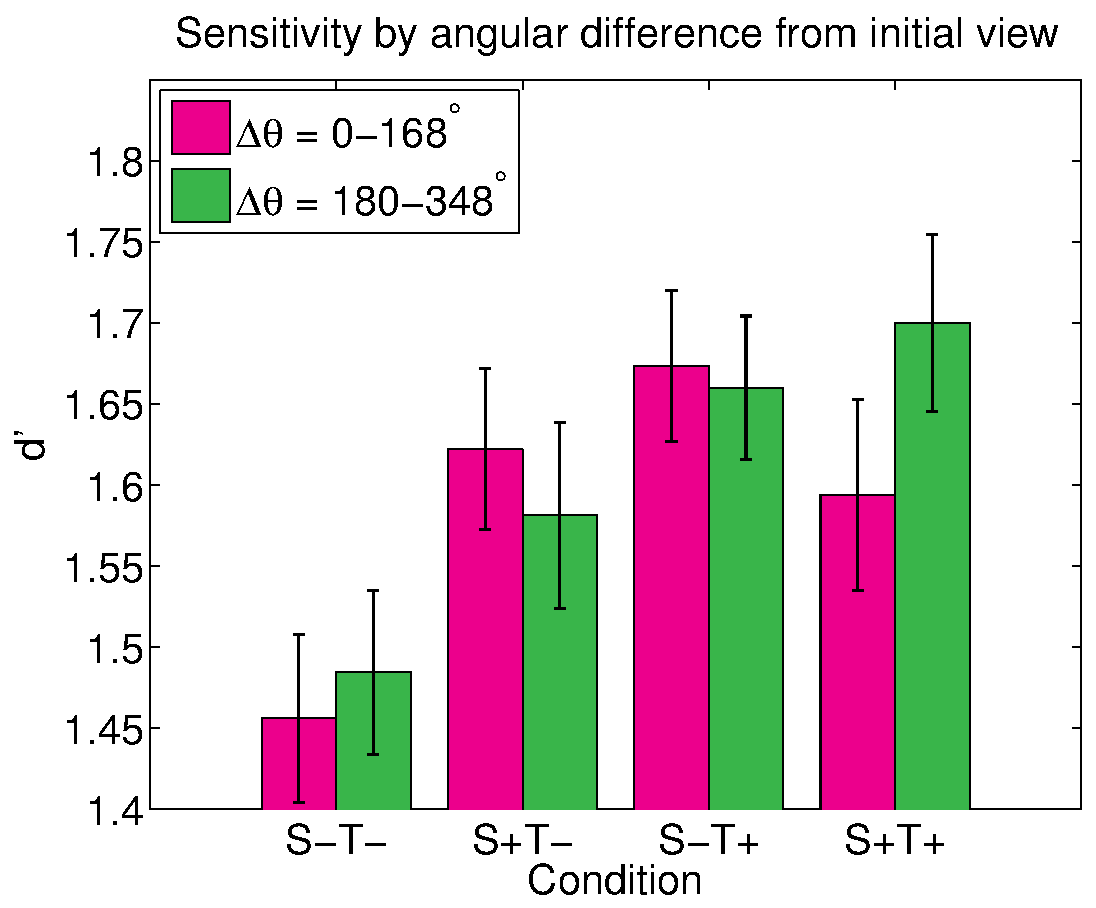
\includegraphics[width=80mm]{figs/chap_pleast/results_dprime_angle.pdf} \\
%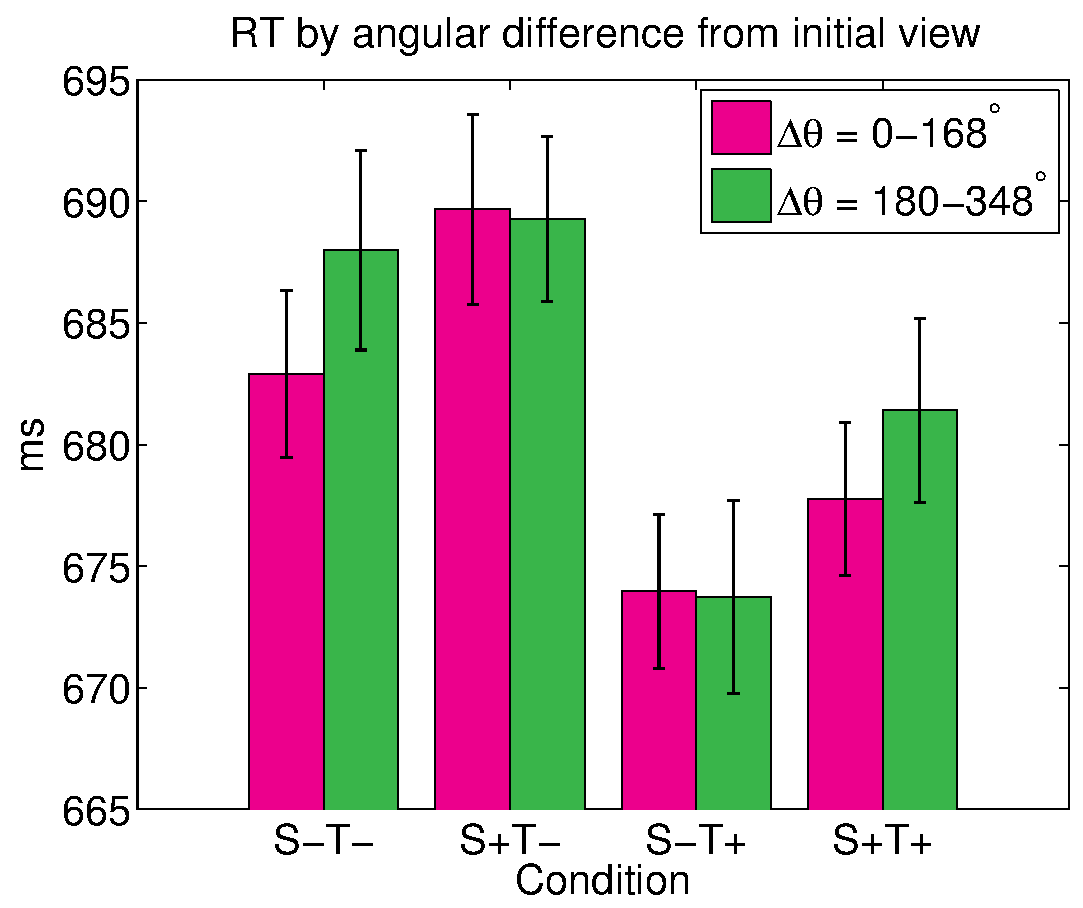
\includegraphics[width=80mm]{figs/chap_pleast/results_rt_angle.pdf} & 
%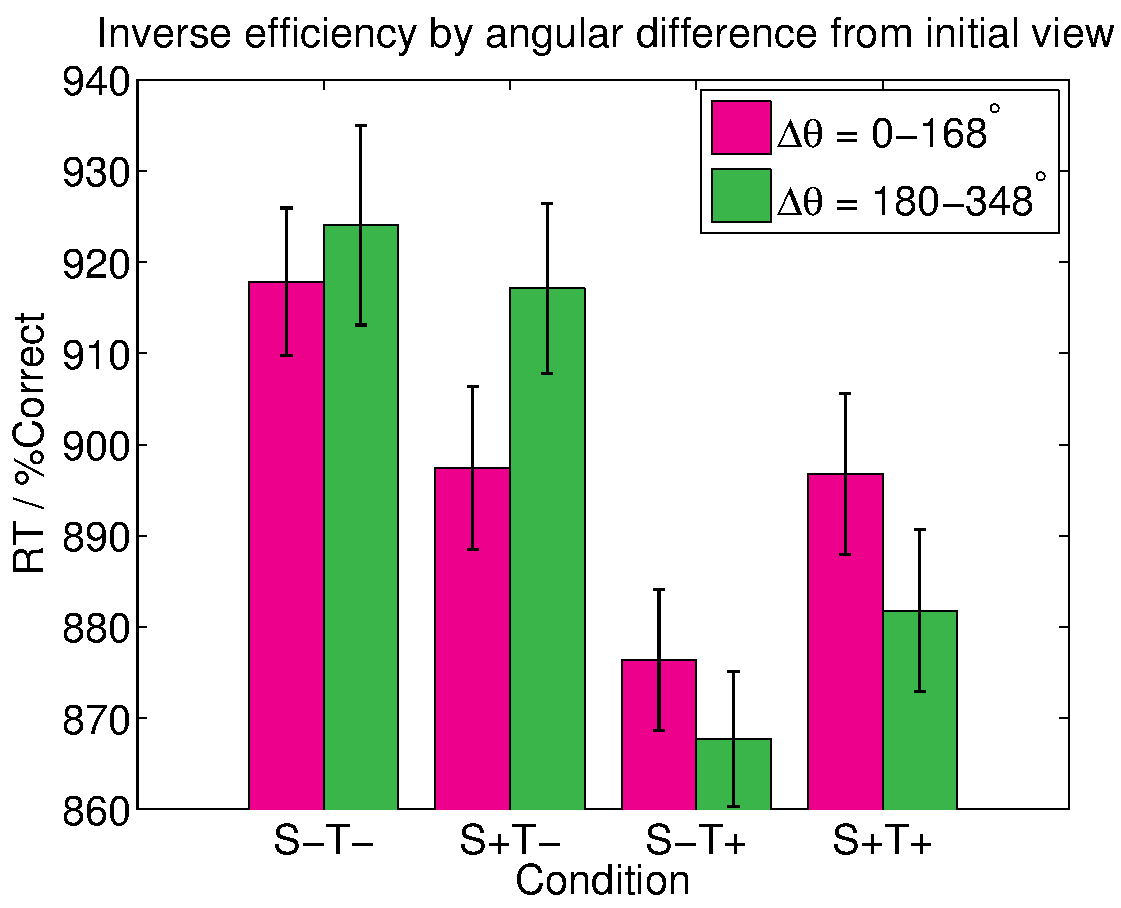
\includegraphics[width=80mm]{figs/chap_pleast/results_ie_angle.pdf} \\
%\end{tabular}
%\caption{Behavioral measures for view interpolation versus extrapolation.}{}
%\end{figure}

\subsection{Time course of spatial and temporal predictability}
A total of five subjects were excluded from EEG analysis -- three for an overabundance of artifacts in the EEG recording resulting in low trial counts after rejection and two for accuracy 2.7$\sigma$ (or further) below mean accuracy across subjects (these two subjects were also excluded from behavioral analyses, see preceding section). The remaining 24 subjects were included in all EEG analyses. 

A 2x2 ANOVA with spatial and temporal predictability as within-subjects factors was used to assess statistical significance at each time bin of event-related averages. \textit{p}-values were corrected for a maximum false discovery rate (FDR) of 5\% using the method described in \incite{BenjaminiYekutieli01}. Additionally, effects were only considered significant if they persisted for at least 16 ms.

To investigate the build-up of spatial and temporal predictability over the entraining sequence, activity from the second through final entraining views was averaged for each condition (the first entraining view is unpredictable, so it is omitted from the average). The results of this analysis are plotted in Figure \ref{fig:pleast_entrain_tla}. The first thing worth noting is that a large 10 Hz periodicity is present for the temporally predictable conditions (S-T+ and S+T+), phase-aligned approximately to the onset of each entrainer. Temporally unpredictable entrainers (S-T- and S+T-) are also approximately periodic. The reason for the 10 Hz periodicity in these conditions despite being temporally unpredictable is likely due to the 750 ms constant duration of the entraining sequence regardless of condition (Figure \ref{fig:pleast_task}B). Presenting eight stimuli in 750 ms with a variable ISI is a 10 Hz presentation rate on average. Still, the temporally unpredictable entrainers exhibit markedly weaker amplitude and are approximately 180 degrees out of phase with the the temporally predictable entrainers.

% erp - entrain
\begin{figure}[h!]
\begin{center}
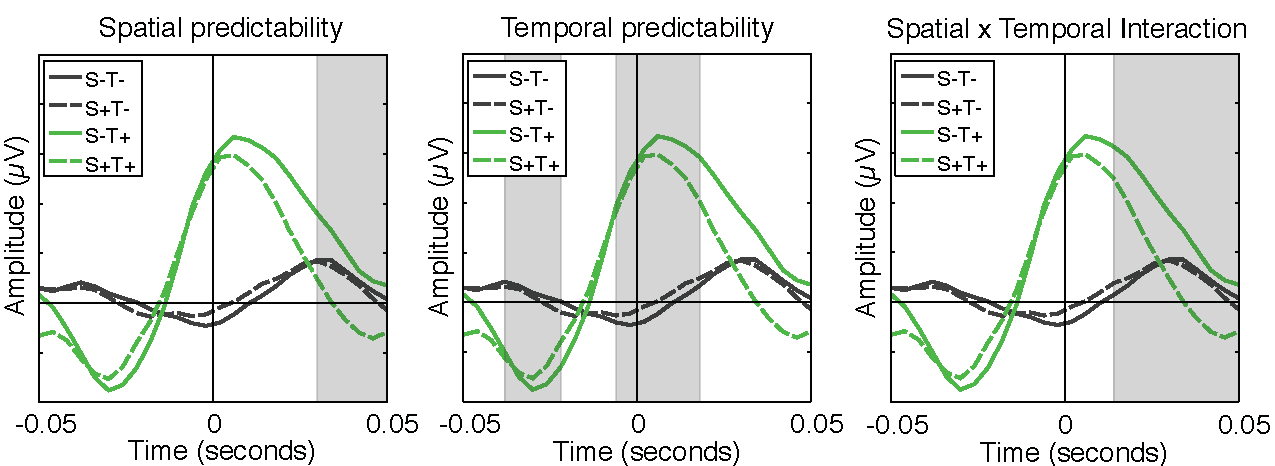
\includegraphics[width=160mm]{figs/chap_pleast/results_entrain_tla_All_montage.pdf}
\end{center}
\caption{Entrainer-evoked activity}{Grand averages for entrainers 2 through 8 as a function of entrainment condition. S-/+ refers to spatially unpredictable and predictable, T-/+ to temporally unpredictable and predictable. All plots depict the grand average with gray shaded regions denoting significant effects of spatial predictability (left), temporal predictability (center), and the interaction between these terms controlling for a maximum false discovery rate (FDR) of 5\%.}
\label{fig:pleast_entrain_tla}
\end{figure}
% revision todo: recreate these figs with y-axis numbers

The effect of spatial predictability manifested 26 ms after the onset of the entrainer and persisted for at least another 24 ms (one quarter of the 10 Hz period). Temporal predictability, in contrast, manifested prior to (-38 through -22 ms pre-stimulus) and at the onset of the entrainer (-6 ms pre-stimulus through 18 ms post-stimulus). The effect of temporal predictability appears to be driven by the antiphase relationship between T- and T+ conditions at these time points. Together, these effects demonstrate differential time courses for spatial and temporal predictability.

Spatial predictability was enhanced when stimuli were temporally predictable. This effect is characterized by the significant interaction between spatial and temporal predictability starting 14 ms after the onset of the entrainer and persisting for at least another 36 ms. This result indicates that the brain is more capable of differentiating between spatially coherent and random sequences of stimuli when it can properly anticipate the presentation of each stimulus (S-T+ versus S+T+) compared to when the onset is unpredictable.

To investigate the effect of spatial and temporal predictability on perception of the probe, waveforms were aligned to the probe onset onset averaged from 200 ms before through 400 ms after (Figure \ref{fig:pleast_probe_tla}). The results of this analysis essentially mirror the entrainer-evoked effects albeit with a few key differences. Temporal predictability was again a purely anticipatory process, manifesting within the pre-stimulus period (-184 ms through -160 ms and -132 ms through -108 ms pre-stimulus). Spatial predictability also manifested briefly within the pre-stimulus period (-128 ms through -80 ms pre-stimulus), which was not seen for spatially predictable entrainers. The post-stimulus effects of spatial predictability occurred much earlier than for entrainers and persisted much longer, beginning approximately at the onset of the probe (-12 ms pre-stimulus) and lasting 136 ms through the P1 response with several transient effects after.

% erp - probe
\begin{figure}[h!]
\begin{center}
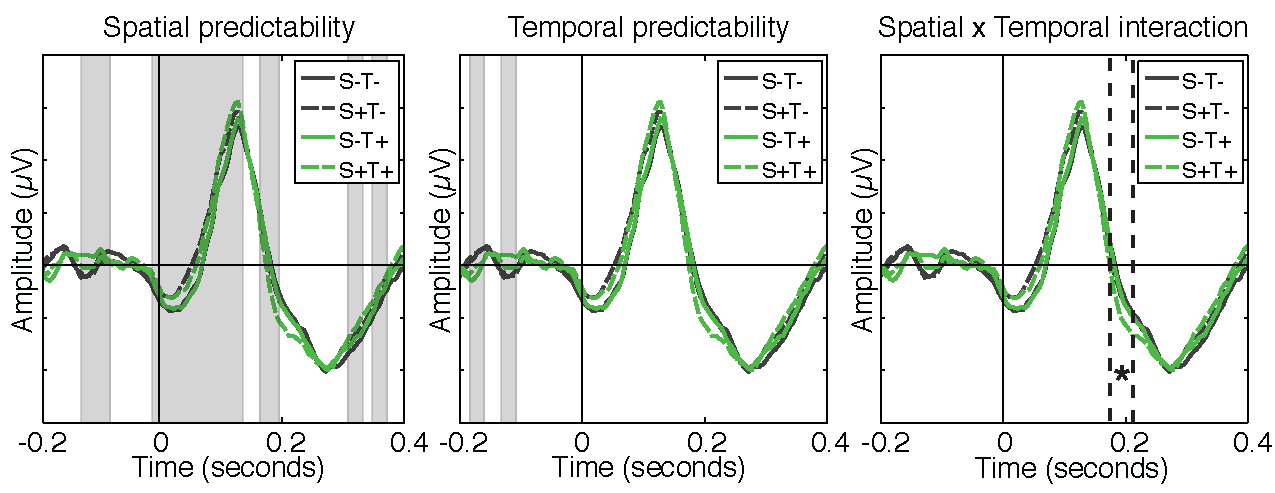
\includegraphics[width=160mm]{figs/chap_pleast/results_probe_tla_All_montage.pdf}
%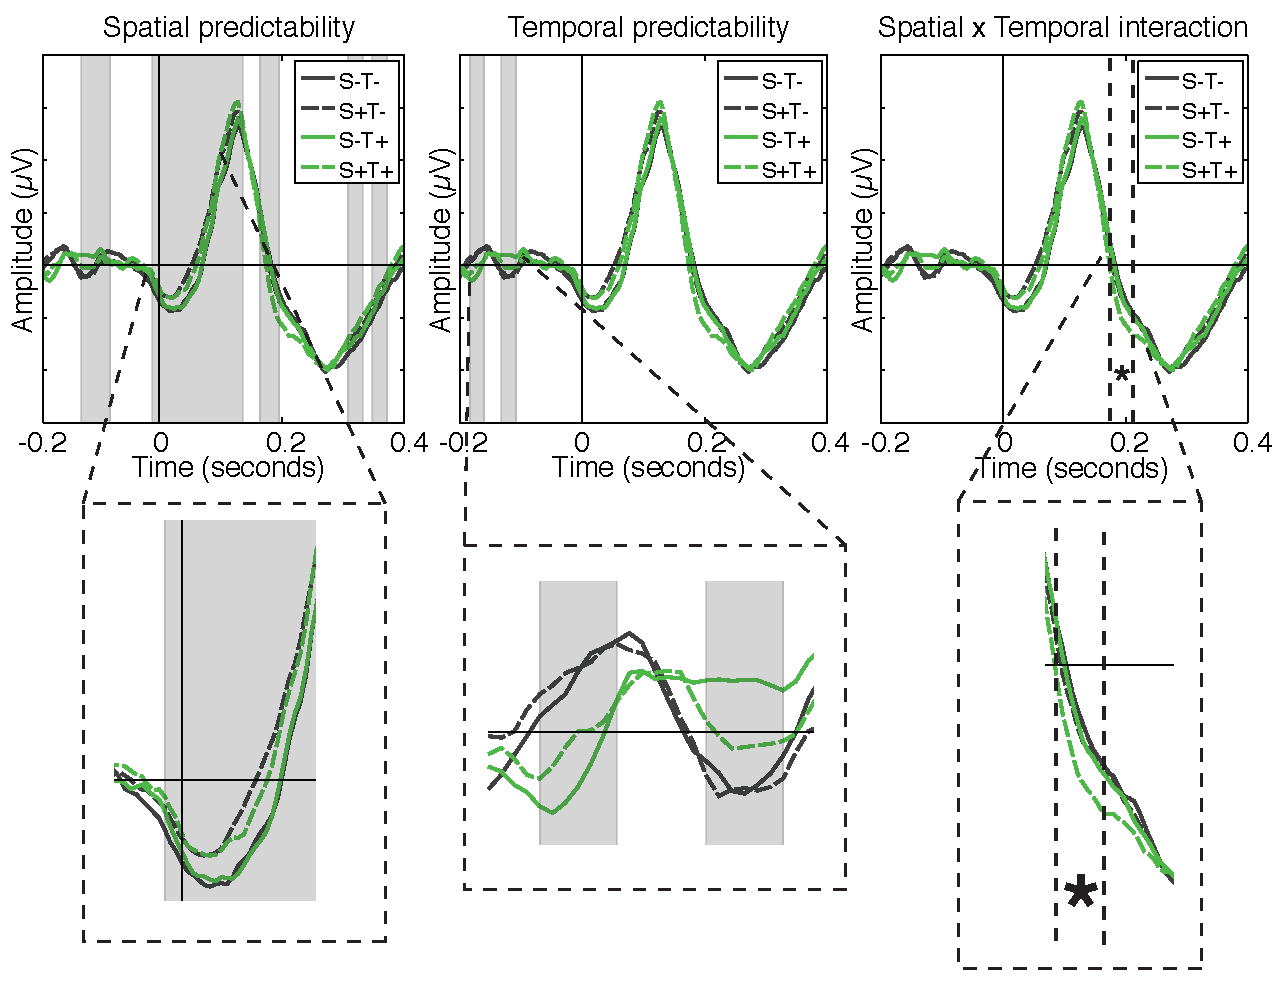
\includegraphics[width=160mm]{figs/chap_pleast/results_probe_tla_All_montage_zoom.pdf}
\end{center}
\caption{Probe-evoked activity}{Grand averages for the probe stimulus, including the preceding 200 ms blank. Asterisk in the interaction plot indicates trending significance at the 5\% level when averaging amplitude within the window defined by the dotted lines.}
\label{fig:pleast_probe_tla}
\end{figure}
% revision todo: recreate these figs with y-axis numbers

Unlike the significant interaction between spatial and temporal predictability for entrainers, the interaction for the probe failed to reach significance given the constraints of the statistical test (maximum FDR of 5\%, 16 ms consecutive significance). However, averaging the amplitude within a window defined by exploratory analysis indicated a trending interaction from 170 ms to 210 ms (\textit{F}(1, 22) = 3.97, \textit{p} = 0.059). This effect was more pronounced and reached significance if only the right hemisphere channels were considered (\textit{F}(1, 22) = 5.61, \textit{p} = 0.027), but failed to reach significance in the left hemisphere (\textit{F}(1, 22) = 2.24, \textit{p} = 0.148), explaining the trending effect when both hemispheres are considered jointly.

\subsection{Predictability entrains alpha oscillations}
The same 24 subjects used in event-related analyses (see preceding section) were used in time-frequency analyses described here. Statistical methods were also identical, consisting of a 2x2 ANOVA with spatial and temporal predictability as within-subjects factors and \textit{p}-values were corrected for a 5\% maximum FDR \cite{BenjaminiYekutieli01}. Effects were only considered significant if they persisted for at least 16 ms.

Power and inter-trial coherence (ITC), a measure of phase angle consistency across trials \cite{LachauxRodriguezMartinerieEtAl99} were computed over a 5-20 Hz frequency range to investigate the relationship between entrainer predictability and alpha oscillatory properties (Figures \ref{fig:pleast_entrain_pow_10Hz}-\ref{fig:pleast_entrain_ITC_10Hz}). Both spatial and temporal predictability had a significant effect on 10 Hz power and ITC beginning around 200 ms after the onset of the first entrainer (power: 160-168 ms after entrainer 1; ITC: 136-208 ms after entrainer 1). Together, these results indicate that 10 Hz entrainment affects both power and phase alignment and takes around 2-3 events to establish. Spatial predictability had a suppressive effect on 10 Hz power and phase alignment whereas temporal predictability had a positive effect. Any interactions between spatial and temporal predictability failed to reach significant levels altogether.

% 10 hz entrain pow
\begin{figure}[h!]
\begin{center}
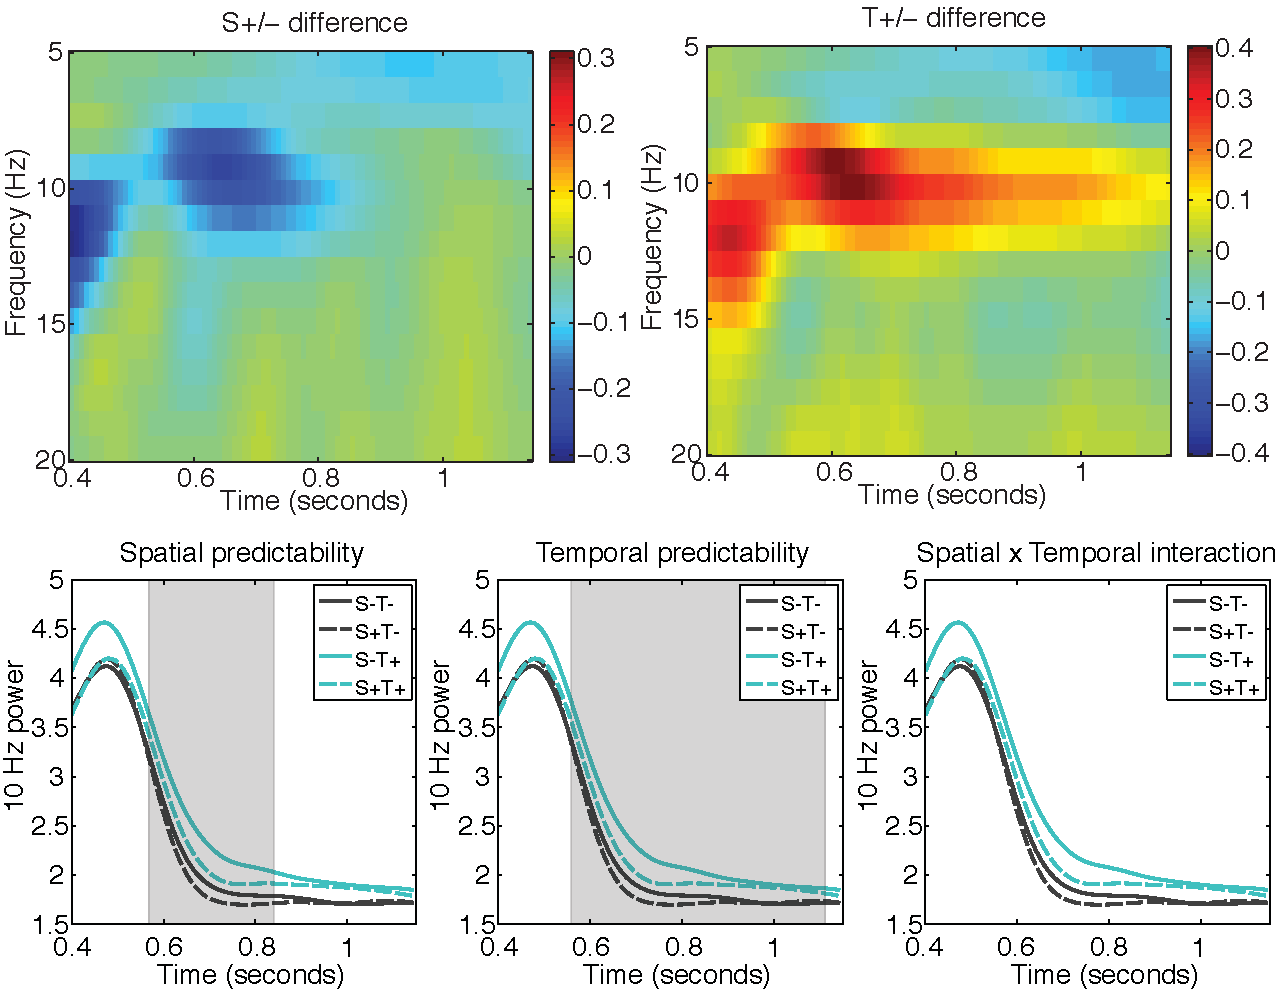
\includegraphics[width=160mm]{figs/chap_pleast/results_powphase_entrain_pow_montage.pdf}
\end{center}
\caption{Effect of entrainer predictability on alpha power}{Alpha-band power over the entraining sequence. \textbf{Top:} Main effects of spatial and temporal predictability on oscillatory power in the 5-20 Hz frequency range. \textbf{Bottom:} 10 Hz only effects of spatial predictability (left), temporal predictability (center), and the interaction between these terms with gray shaded ranges indicating significance while controlling for a maximum false discovery rate (FDR) of 5\%. S-/+ refers to spatially unpredictable and predictable, T-/+ to temporally unpredictable and predictable. Time axes indicate total trial time after the initial fixation cross with 0.4 seconds corresponding to the first entrainer.}
\label{fig:pleast_entrain_pow_10Hz}
\end{figure}

% 10 Hz entrain ITC
\begin{figure}[h!]
\begin{center}
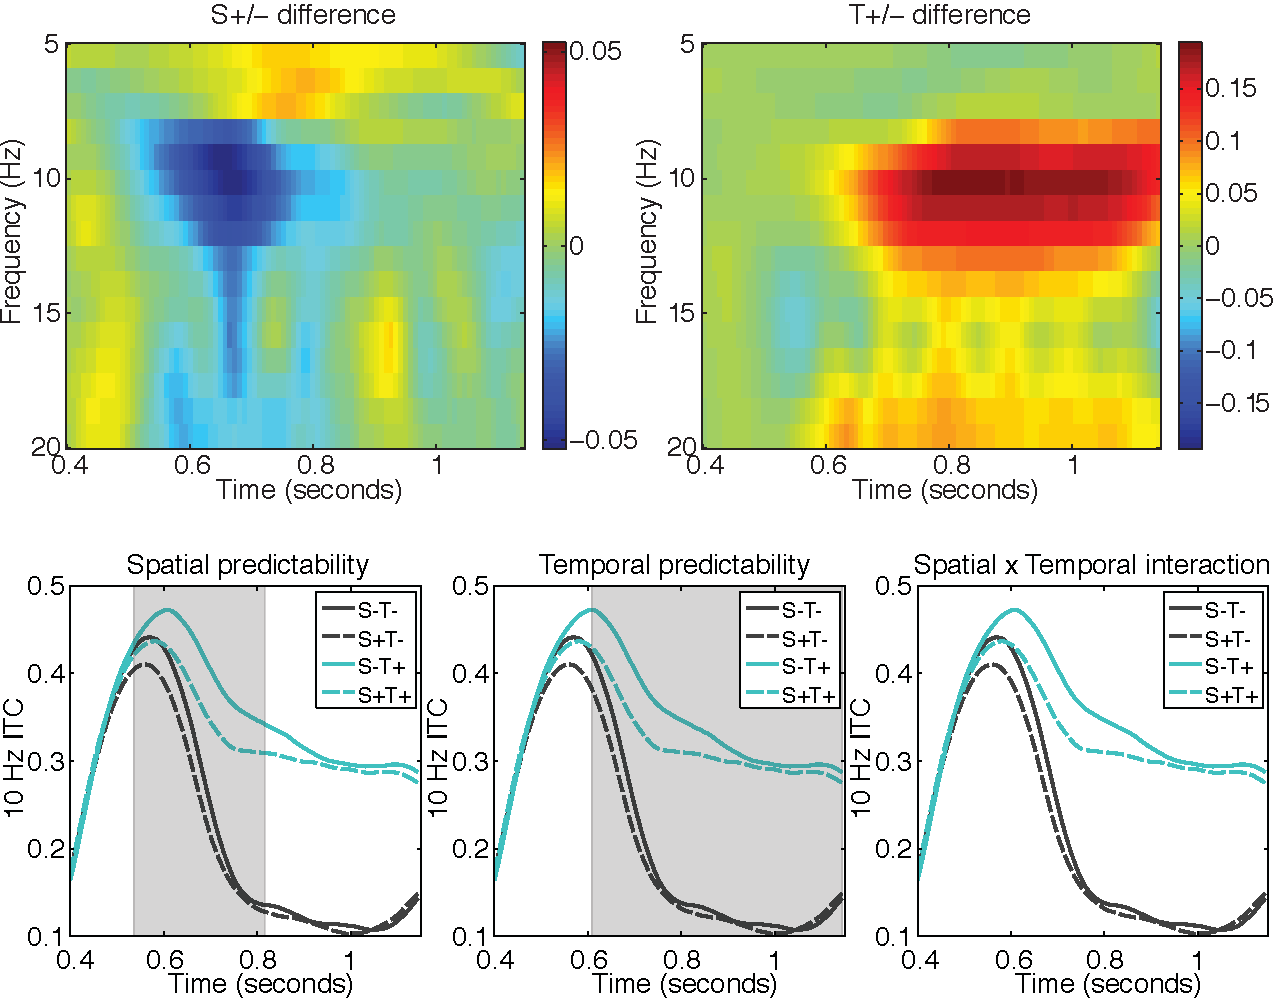
\includegraphics[width=160mm]{figs/chap_pleast/results_powphase_entrain_ITC_montage.pdf}
\end{center}
\caption{Effect of entrainer predictability on alpha phase coherence}{Alpha-band inter-trial coherence (ITC) over the entraining sequence. Axes, legends, and shading for significant regions are the same as those described in Figure \ref{fig:pleast_entrain_pow_10Hz}.}
\label{fig:pleast_entrain_ITC_10Hz}
\end{figure}

The effect of spatial predictability only persisted for three entrainers on average (duration ranges for 10 Hz power and ITC: 272-280 ms). Temporal predictability, in contrast, exhibited a sustained effect on 10 Hz power lasting nearly the entire entraining sequence. In the case of ITC, the effect of temporal predictability persisted throughout the blank period that separated the entraining sequence and the probe (Figure \ref{fig:pleast_probe_ITC_10Hz}). This result indicates that alpha phase remained more aligned for temporally predictable stimuli even without exogenous entrainment. 

Predictability effects on 10 Hz ITC failed to reach significance during the presentation of the probe or the following 400 ms period given the constraints of the statistical test (maximum FDR of 5\%, 16 ms consecutive significance). An enhancement in ITC could be observed for the combined predictability (S+T+) condition and trended toward significance when averaged over a 100 ms period beginning 155 ms after the onset of the probe (\textit{F}(1, 22) = 4.11, \textit{p} = 0.055). This effect was more pronounced and reached significance if only the right hemisphere channels were considered (\textit{F}(1, 22) = 7.45, \textit{p} = 0.012), but failed to reach significance in the left hemisphere (\textit{F}(1, 22) = 1.47, \textit{p} = 0.237), explaining the trending effect when both hemispheres are considered jointly. 

% 10 Hz probe ITC
\begin{figure}[h!]
\begin{center}
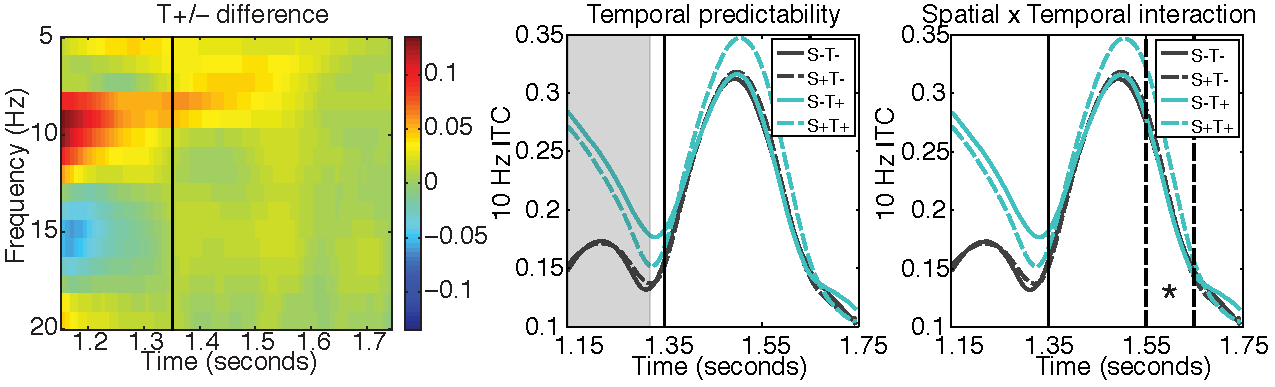
\includegraphics[width=160mm]{figs/chap_pleast/results_powphase_probe_ITC_montage.pdf}
\end{center}
\caption{Alpha phase coherence before and after probe}{Alpha-band inter-trial coherence (ITC) 200 ms preceding the probe and 400 ms following. Solid vertical line indicates probe onset. Asterisk indicates trending significance at the 5\% level when averaging 10 Hz ITC within the window defined by the dotted lines. Time axes indicate total trial time after the initial fixation cross.}
\label{fig:pleast_probe_ITC_10Hz}
\end{figure}

\subsection{Predictability effects in delta-theta bands}
The effects of spatial and temporal predictability on oscillatory properties during the probe period (-200 ms pre-stimulus through 400 ms after) were investigated in the delta-theta bands, centered around 5 Hz. This frequency was identified based on exploratory analysis and was also motivated by alternative models of sensory prediction \cite[e.g.,]{ArnalGiraud12,GiraudPoeppel12}. Power and ITC at 5 Hz are plotted in Figures \ref{fig:pleast_probe_pow_5Hz}-\ref{fig:pleast_probe_ITC_5Hz}.

% 5 Hz probe pow
\begin{figure}[h!]
\begin{center}
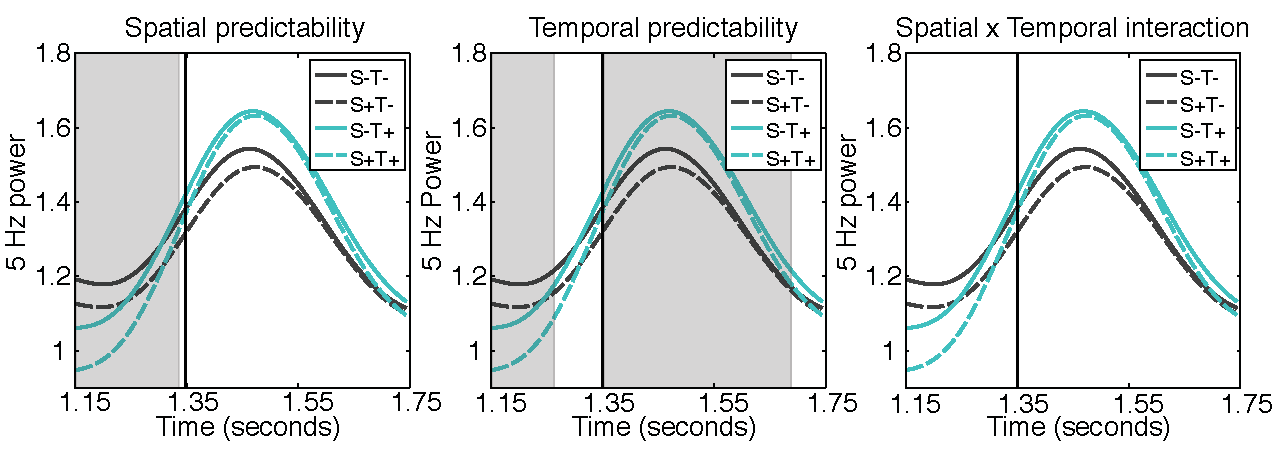
\includegraphics[width=160mm]{figs/chap_pleast/results_powphase_probe_5Hz_pow_montage.pdf}
\end{center}
\caption{Delta-theta power before and after probe}{Delta-theta power 200 ms preceding the probe and 400 ms following. Axes, legends, and shading for significant regions are the same as those described in Figure \ref{fig:pleast_probe_ITC_10Hz}.}
\label{fig:pleast_probe_pow_5Hz}
\end{figure}

% 5 Hz probe ITC
\begin{figure}[h!]
\begin{center}
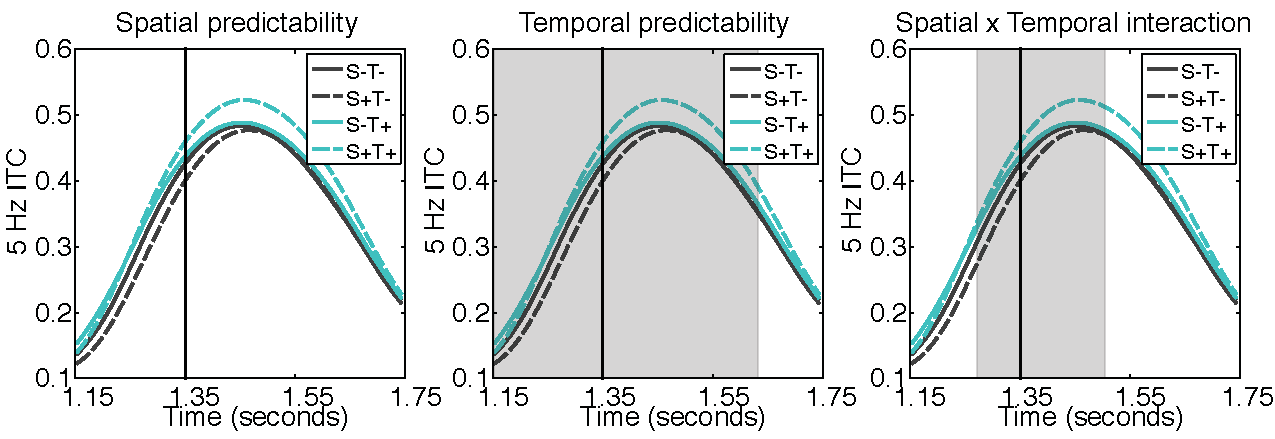
\includegraphics[width=160mm]{figs/chap_pleast/results_powphase_probe_5Hz_ITC_montage.pdf}
\end{center}
\caption{Delta-theta phase coherence before and after probe}{Delta-theta inter-trial coherence (ITC) 200 ms preceding the probe and 400 ms following. Axes, legends, and shading for significant regions are the same as those described in Figure \ref{fig:pleast_probe_ITC_10Hz}.}
\label{fig:pleast_probe_ITC_5Hz}
\end{figure}

Both spatial and temporal predictability had a significant effect on 5 Hz power during the 200 ms blank period preceding the probe. Temporal predictability had a  suppressive effect on 5 Hz power, in contrast to the positive modulation found for 10 Hz power. This effect reversed following the presentation of the probe and persisted for over 300 ms. The interaction between spatial and temporal predictability failed to reach significance for 5 Hz power at any time points.

Temporal predictability also had a significant effect on 5 Hz ITC beginning during the 200 ms blank period preceding the probe and lasting nearly 300 ms after the presentation of the probe. Whereas 10 Hz ITC decreased during the blank period (yet remained significantly higher for temporally predictable stimuli), 5 Hz ITC increased, and continued to increase until approximately 100 ms after the onset of the probe. 5 Hz ITC was highest for the combined spatial and temporal predictability condition (S+T+), indexed by a significant interaction beginning before the probe onset (-78 ms pre-stimulus) and persisting 154 ms after.

% \subsection{Predictability effects in gamma oscillations}
% 35 Hz int ???

%\subsection{Alpha phase at probe onset}

\section{Discussion}

\subsection{Summary of results}

The work described in this chapter investigated how the brain integrates information from 100 ms samples and uses it to drive predictions about what will happen. The experimental paradigm used to address this question involved entraining alpha oscillatory activity to determine the effects of spatial and temporal predictability on a novel object recognition task. Behaviorally, there were robust effects of temporal predictability on raw accuracy and reaction times, as well as transformations to \textit{d'}, a measure of sensitivity that takes into account response bias, and inverse efficiency, a measure that combines accuracy and reaction times \cite{TownshendAshby78}. Accuracy was higher and response times were faster for a same-different judgement when entraining stimuli were presented in a temporally predictable manner. Spatial predictability was only significant for \textit{d'} scores with higher sensitivity between ``same'' and ``different'' probes when entraining stimuli were presented in a predictable order, suggesting that raw accuracy might have been contaminated by response bias. Inverse efficiency, which can be thought of as the amount of energy consumed by the system to produce a behavioral outcome \cite{TownshendAshby83}, was lower for temporally predictable stimuli on average, but exhibited an increase for combined spatial and temporal predictability.

Event-related analysis of EEG data indicated that temporal predictability causes a strong periodicity (in this case, 10 Hz) phase aligned approximately to the onset of each temporally predictable entraining stimulus. This alignment approximately 180 degrees out of phase for temporally unpredictable stimuli and these differences in waveform alignment caused amplitude differences that preceded both entraining stimuli and the probe. The effects of spatial predictability generally manifested during the presentation of stimuli. There was an early divergence of probe-evoked activity caused by spatially predictable ordering of entrainers that over 100 ms through the P1 response with several transient effects after. There was evidence that spatial predictability was only effective when stimuli were also temporally predictable. This was evident for entrainers, and over right hemisphere channels during the probe. The effect failed to reach significance for left hemisphere channels and only trended toward significant levels when both hemispheres were considered jointly. It is likely that this is simply an issue of insufficient power, but other explanations such as hemispheric specialization \cite[e.g.,]{Dien09b} cannot be completely ruled out.

Both spatial and temporal predictability had effects on the power and phase coherence (indexed by inter-trial coherence, ITC) of neural oscillations. Spatially predictable entrainment caused a suppression of 10 Hz power with a lower degree of phase alignment than spatially random stimuli. Temporally predictable entrainment had the opposite effect, with increased 10 Hz power and phase alignment. Phase alignment due to temporal predictability remained elevated compared to temporally unpredictable stimuli during a 200 ms blank period between the entraining sequence and probe, indicating phase alignment could persist without exogenous entrainment. There was evidence of selective an enhancement in phase alignment for the combined spatial and temporal predictability case. As was the case in event-related analyses, this effect was significant in the right hemisphere, but not the left, and trended toward significance when both hemispheres were considered jointly. Power and phase coherence effects were also examined in the delta-theta bands (5 Hz) during the probe judgement. Results were similar to those found for 10 Hz, but more robust with effects for both power and phase alignment. 

\subsection{Separate time courses for spatial and temporal prediction}
Spatial and temporal predictability were characterized by distinct and generally non-overlapping time courses. Temporal predictability manifested solely before (or at) the onset of each stimulus and appeared to be driven by an approximate antiphase relationship between temporally predictable and unpredictable stimuli. Spatial predictability generally manifested during the presentation of stimuli, although in the case of the probe, showed transient difference without stimulation. Predictability effects were similar for entraining stimuli and the probe except that the effect of spatial predictability persisted for over 100 ms through the P1 response with several more transient effects after. The similarity between entrainers and the probe suggests that the brain might treat the probe as a continuation of the entraining sequence and process it in the same manner. 

From these results, we can conclude that temporal prediction is an anticipatory process, occurring during the absence of exogenous stimulation (in between entrainers or before the probe). The effect of temporal predictability extends 16 ms after the onset of each entrainer, but latencies for the first wave of responses in primary visual cortex (V1) are approximately 40-60 ms \cite{NowakBullier97,FoxeSimpson02} so there is no exogenous stimulation \textit{per se} during the duration of the effect despite the stimulus being onscreen. Spatial prediction begins shortly before exogenous stimulation, but in the case of the probe, persists through the initial V1 responses. Spatial prediction, thus, might better be characterized as a post-stimulus process opposed to truly anticipatory process. The computation might involve a comparison between what is expected and what is actually coded by incoming spikes, consistent with the LeabraTI model (Chapter \ref{chap:leabrati}) as well as predictive coding models \cite[e.g.,]{RaoBallard99}.

% * previous studies by \cite{DohertyRaoMesulamEtAl05,RohenkohlNobre11}. or wait until the ``not attention'' section?
% FurlVanRijsbergenKiebelEtAl10 -- some MEG stuff on predictability

\subsection{Oscillatory mechanisms of spatial and temporal prediction}
Spatial and temporal predictability had effects on both power and phase coherence of neural oscillations. In both cases, predictability took 2-3 entraining stimuli to establish, consistent with previous investigations (\nopcite{MathewsonFabianiGrattonEtAl10}; \abbrevnopcite{MathewsonPrudhommeFabianiEtAl12}). Spatial predictability was then characterized by a suppression of 10 Hz power and a phase angle variability causing a lower degree of alignment than spatially random stimuli. This effect is opposite than that of temporal predictability, which was characterized by increased 10 Hz power and phase angle alignment. Previous investigations have generally not simultaneously manipulated temporal rhythmicity and spatial coherence \cite[although see]{DohertyRaoMesulamEtAl05} and thus, the relative suppression and decreased phase coherence during spatially predictable entrainment were unexpected results.

Successful oscillatory entrainment is thought to be a result of repeated phase resetting of endogenous oscillations causing phase to move into alignment with the frequency of exogenous stimulation \cite{SchroederLakatosKajikawaEtAl08,CalderoneLakatosButlerEtAlInPress}. Oscillatory phase resetting has been shown to be caused by salient, unexpected events (\abbrevnopcite{FiebelkornFoxeButlerEtAl11}; \nopcite{LandauFries12,RomeiGrossThut12}) and thus these unexpected results might be accounted for by considering successive views in terms of the amount of ``surprise'' \cite{IttiBaldi09,MeyerOlson11} they evoke. Subsequent views of the entraining sequence have significant feature overlap, characterized by the same populations of neurons spiking from one view to the next. Repeated spiking, especially as a function of expectation, has been shown to evoke rate suppression mechanisms \cite{SummerfieldTrittschuhMontiEtAl08}. When entraining views are presented out of order, feature overlap is minimized and each view is ``surprising'', causing an initial fast spiking burst response, which could lead to a higher degree of phase resetting.

The entrainment effects of spatial predictability were transient and dissipated before the end of the entraining sequence whereas the effects of temporal predictability persisted much longer. This might account for the null effects of spatial predictability on most behavioral measures. Temporal predictability effects persisted through the 200 ms blank period between the entraining sequence and probe and had robust effects on all behavioral measures. Thus, the present experiment could be modified to use a shorter entrainment sequence which would likely elicit successful spatial predictability for probe judgements.

The enhancement of 10 Hz phase angle alignment after the probe was presented did not reach significant levels assuming the FDR-corrected significance test at each time bin but did for 5 Hz phase alignment. Furthermore, temporal and spatial predictability main effects around the probe onset were more pronounced for 5 Hz oscillatory properties. One potential explanation for these effects is that reason for this is that the 200 ms blank period between the entraining sequence and the probe corresponded to two cycles at 10 Hz, but only on cycle at 5 Hz. Phase angles at 10 Hz exhibited significant dealignment over this period, and actually increased in alignment at 5 Hz. Thus, it is possible that this increase in phase alignment lead to a more pronounced selective enhancement for combined spatial predictability at 5 Hz, consisted with recent data \cite{CravoRohenkohlWyartEtAl13}. A more robust effect might be found for 10 Hz if the blank period between the entraining sequence and probe was only 100 ms in duration.

Another limitation of the present experimental paradigm is that it is unclear whether exogenous entrainment simply created new oscillations akin to steady state visually evoked potentials (SSVEP), or actually entrained existing endogenous oscillations. Thus, it might not be particularly surprising that temporally predictable stimuli caused increases in power and phase alignment. However, entrained alpha-band periodicity has been shown to correlate with individual resting alpha oscillation frequency \abbrevcite{DeGraafGrossPatersonEtAl13} so it is likely that the paradigm recruited existing oscillations and caused them to align to the exogenous entrainment frequency. The fact that phase alignment continued through the 200 ms blank period without exogenous entrainment also supports this claim.


\subsection{Prediction is not simply attentional orienting}
TODO after writing intro
% maybe hold off on tieing effects into pref literature (nobre, etc.) until here

% relation btwn o/c and behave effects
% * 5 Hz Super bonus related to IE since it is the only cross-over interaction
% * 5 Hz pow related to accuracy? seems plausible, follows same order

% de graaf sees performance oscillation for 5 Hz too

\subsection{Why does combined spatial and temporal predictability increase inverse efficiency?}

% Discussion outline
%
% Behavioral results
% * generally always signif effect of temporal (acc, d', rt, ie)
% * spatial only significant for d'
% * no synergistic effect of S+T+, just large improvements from S-T-
% * IE crossover interaction mystery -- why is it even important?

%%%
% save for general discussion
%%%
% * LeabraTI: why do low frequency oscillations convey information about spatial predictability
%	  % Low frequency oscillations seem to capture spatial stuff too, not just temporal stuff although it's hard to know for sure without a better expt
%
%	  % 5 Hz better for temporal prediction time window than 10 Hz? Again, at least given current data, but hard to know
% * 5 Hz vs 10 Hz
% *		Is 5 Hz functionally different? Or just a subharmonic that is better suited for significance given the experimental parameters (200 ms blank)
%
% Stronger 10 Hz effects without attention

\bibliographystyle{apa}
\bibliography{ccnlab}
\end{document}